\section{Oppgaver uke 6}

\subsection{Assignment 1} 

First off, I'd like to state that I was extremely confused as to the objectives of this assignment, so these answers may be completely off, but ...

\begin{enumerate}
	\item The statistics show that the amount of players is always lower than 44876, and with a 94.73\% chance it will be higher than 27106. Although the average amount of players is 4311, the player count is with 95\% accuracy between 27106-44876. The 5\% and 1\% charts narrows this down even more, and show us that there's a 99.9\% probability of the player count being lower than 42654. 
	\item Examining the \textit{begin} file and the \textit{end} file, we see that the maximum player count for the former was at around 21000 players, although this wasn't very common. This climbed and reached a maximum number of 30181 in the end.
	\item By knowing the probability a certain amount of players will be online, it's easier to know how much resources should be allocated to the database server. However, without knowing the specific times (as these weren't included), it makes it slightly harder to determine such things as \textbf{when} the peak hours actually occur and compensate with more/less servers (i.e via AWS, where servers can be set to be created and destroyed at specific times to account for increased traffic).
	
\end{enumerate}

\subsection{Assignment 2}

Again, I am pretty unsure about reading the Calc document, but here goes ...
\begin{enumerate}
	\item Done!
	\item Done, using: cat /mysql\_queries\_long | grep select | cut -f3 -d, 
	\item The data here shows that the number of selects are rather consistent and only vary +-9 from 6742
\end{enumerate}

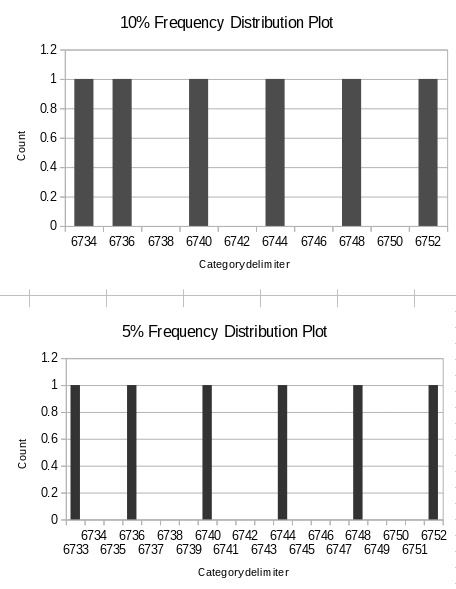
\includegraphics[scale=0.6]{graph.png}
\newpage
\subsection{Assignment 3}
db1 has been dead for quite some time and the data we have to work with isn't very useful for calculating a linear rise and maximal capacity. I began calculating the rise for the data we had, but having just run some stresstests, it was fluctuating between extremes and seemed unreliable.

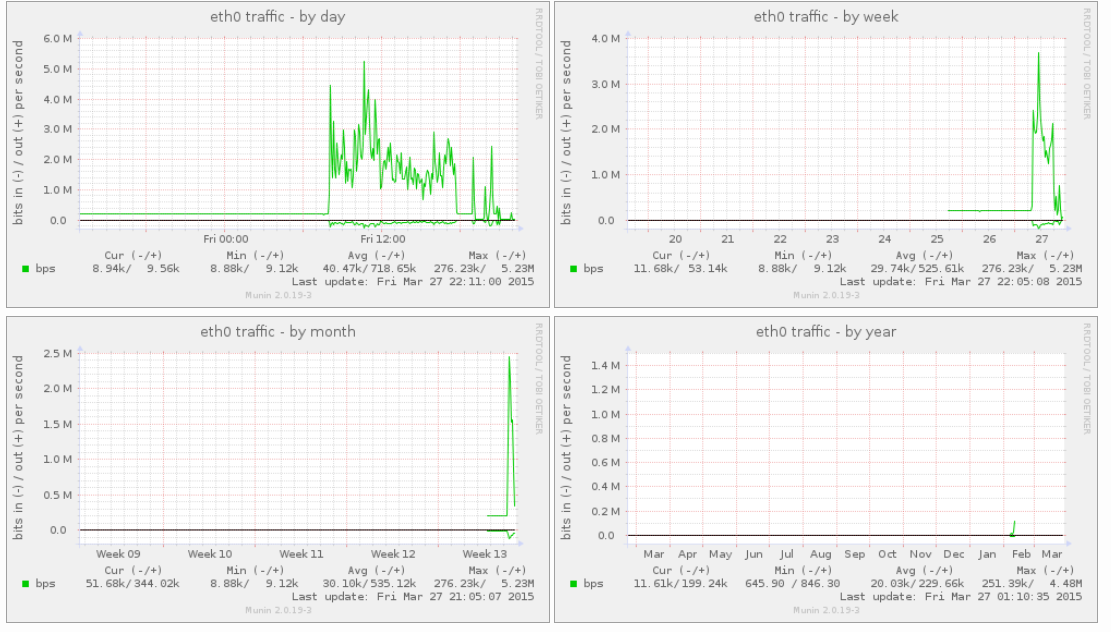
\includegraphics[scale=0.4]{munin.png}